\documentclass[a4papaer]{article}
 
\usepackage{hyperref}
\usepackage[left=1.0cm,top=0.5cm,right=1.0cm,bottom=1.0cm]{geometry}
\usepackage[spanish, english]{babel}
\usepackage[utf8]{inputenc}
\usepackage{amsmath}
\usepackage{nccmath}
\usepackage{graphicx}
\usepackage[colorinlistoftodos]{todonotes}
\usepackage{amssymb}
\usepackage{listings}
\providecommand{\abs}[1]{\lvert#1\rvert}
 
 
\begin{document}
 
\title{Laboratorio 3 Redes de Computadores}
\author{Diego Muñoz - 201073572-9 - diego.munozd@alumnos.usm.cl}
\date{20 de Junio de 2014}
\maketitle
 
\section{Introducción}
 
La resolución de este trabajo se hizo completamente en Latex, desarrollando manualmente los ejercicioes, asi, evitando codigo en python.
 
\section{Usando OVT}
 
Para el desarrollo de esta sección, se utilizó un simil a la aplicacion Open Visual Traceroute, debido a que no se encontraba disponible para MacOSX, esta aplicación se llama Visualroute y se puede encontrar en $http://www.visualware.com/$.

Es sabido que las conexiones intercontinentales son mediante cables submarinos ($http://www.submarinecablemap.com/$), por lo que notaremos que todas las direcciones que probamos en esta tarea primero salen de Chile a Estados Unidos independiente del destino final que estos tengan, esto es debido a que no existe conexion directa con Australia por ejemplo, al abrir la pagina de la embaja de Australia, nos lleva a travez de USA. Esto lo podemos ver en el capítulo 1 del ramo, en donde nos hablan de niveles de internet, ISP1 e ISP2 para conexiones nacionales e internacionales.

\subsection{http://moodle.inf.utfsm.cl/}

\begin{figure}[h]
  \centering
    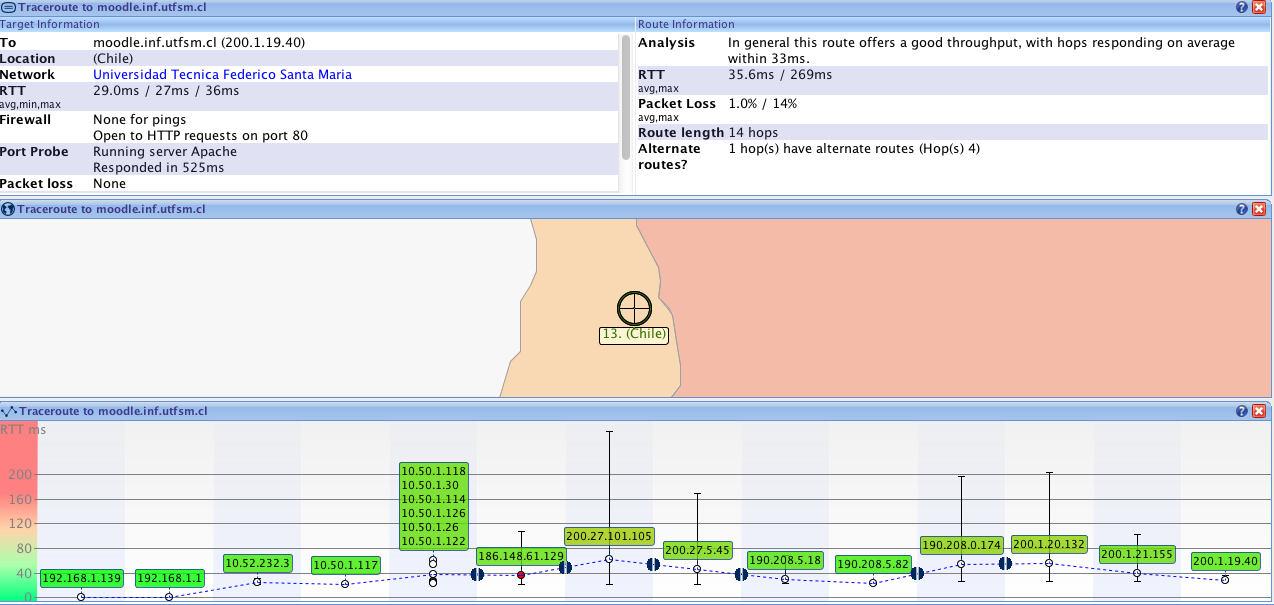
\includegraphics[width=1\textwidth]{ss1}
  \caption{Moodle}
  \label{fig:Trace Route de http://moodle.inf.utfsm.cl/}
\end{figure}


Es el caso ejemplificador de conexiones locales, notamos en la screen que ninguno de los hops por los que pasan los paquetes salen de Chile, esto es debido a que el servidor donde esta alojado Moodle se encuentra en Valparaiso, por lo que, los paquetes eligen la ruta mas optima, que es manteniendos dentro del territorio nacional. Además podemos observar todos los tiempos de respuestas estan en color verde, lo que para la aplicación significa que son optimos, salvo los ultimos 2, que es cuando llegan a los routers en Valpariso que aumentan sus tiempos de respuesta un poco. En resumen, al encontrarse los servidores de destino en la misma red nacional, no requiere una conexión internacional.

\pagebreak

\subsection{http://cime.cl/}


\begin{figure}[h]
  \centering
    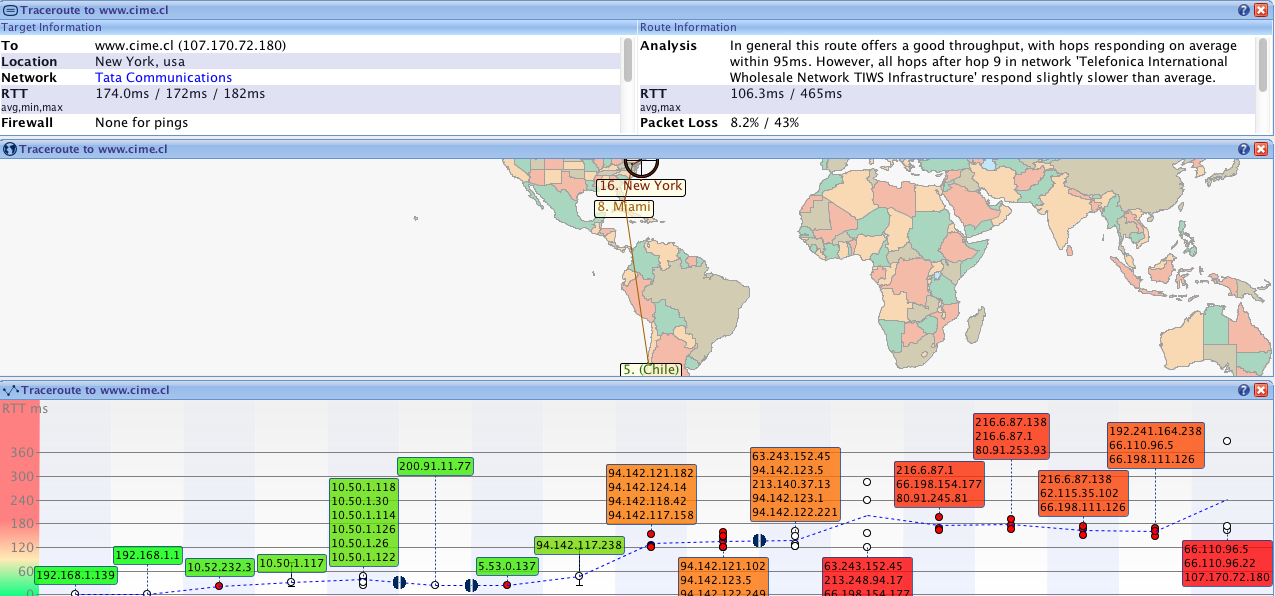
\includegraphics[width=1\textwidth]{ss2}
  \caption{Cime}
  \label{fig:Trace Route de http://cime.cl/}
\end{figure}



Para el caso de cime, notamos que los servidores se encuentran en Nueva York, USA. A diferencia de Moodle, la conexion debe salir de la red chilena y dirigirse a USA, para esto los paquetes llegan a Valparaiso, donde se encuentra la salida al cable submarino, y a travez del enlace internacional  \textbf{Telefónica International Wholesale Network Infrastructure} sale hacia Estados Unidos donde se reciben en Miami. Luego llegado a USA es donde se complica un poco, porque dentro de este país existen muchas redes locales (ISP2), en la cuales los paquetes deben acceder dependiendo el servidor donde esten alojados. En este caso, $cime$ toma la rede \textbf{TATA Communications} hasta su llegada a Nueva York.
 
\begin{figure}[h]
  \centering
    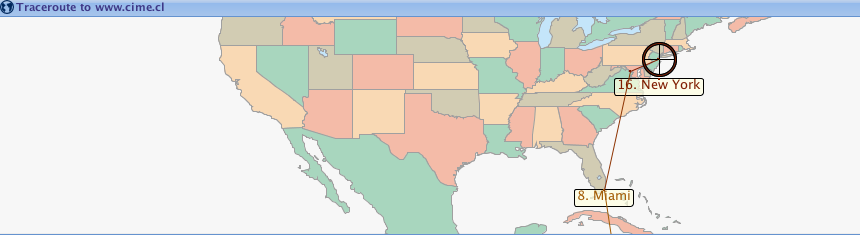
\includegraphics[width=1\textwidth]{ss3}
  \caption{Cime}
  \label{fig:Trace Route de http://cime.cl/}
\end{figure}


\pagebreak

\subsection{http://wikipedia.com/}

\begin{figure}[h]
  \centering
    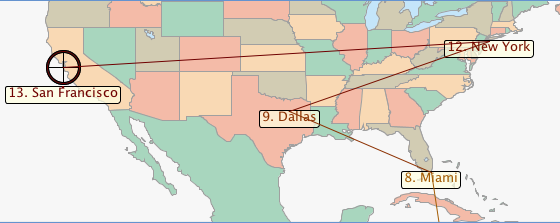
\includegraphics[width=1\textwidth]{ss5}
  \caption{Wikipedia}
  \label{fig:Trace Route de http://wikipedia.org/}
\end{figure}

Notamos que los servidores de Wikipedia estan alojados en la red Wikimedia en San Francisco, USA. Para llegar alla, al igual que en el caso de Cime que esta alojado en Nueva York, los paquetes viajan a travez de la red nacional hasta llegar al punto de salida en valparaiso de \textbf{Telefónica International Wholesale Network Infrastructure} llegando a la misma en Miami. Luego viajan hacia Dallas por la misma red, finalmente para llegar a una de las redes nacionales de USA \textbf{Tinet International Network}. 

\begin{figure}[h]
  \centering
    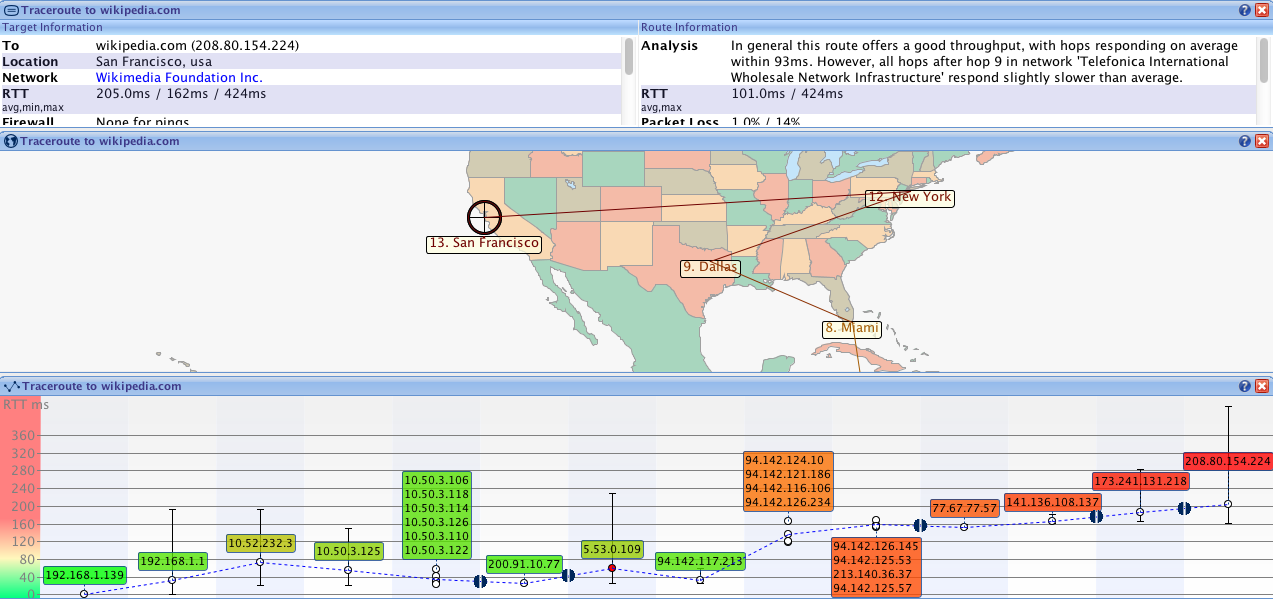
\includegraphics[width=1\textwidth]{ss4}
  \caption{Wikipedia}
  \label{fig:Trace Route de http://wikipedia.org/}
\end{figure}

Una vez mas, notar que los paquetes al salir de territorio nacional (hop 94.142.117.213), aumentan sus latencias en los tiempos de respuesta, mostrandose de color naranjo o rojo, aun despues de escoger las mejores rutas.

\pagebreak

\subsection{http://www.chile.embassy.gov.au/}

\begin{figure}[h]
  \centering
    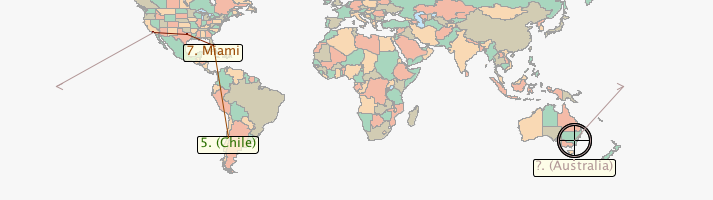
\includegraphics[width=1\textwidth]{au1}
  \caption{Embajada Australia en Chile}
  \label{fig:Trace Route de http://www.chile.embassy.gov.au/}
\end{figure}

A diferencia de los casos anteriores, los servidores de la embajada de Australia en Chile se encuentrán en Australia, por lo tanto, se observan algunos cambios en el camino por el cual los paquetes realizan su camino. Para llegar a Australia, no existe un enlace directo desde Chile, por lo que los paquetes generan su camino hacia Estados Unidos por la ruta de salida de Chile ya mencionada (Telefónica), luego pasa por la rede local de Estados Unidos, \textbf{Level 3 Communications, Inc} hasta la salida a un nuevo cable submarino que atravieza todo el Oceano Pácifico regido por la empresa \textbf{Pacnet Service (Japan)} hasta su llegada a Australia.

\begin{figure}[h]
  \centering
    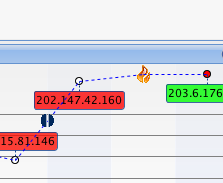
\includegraphics[width=0.5\textwidth]{au4}
  \caption{Embajada Australia en Chile}
  \label{fig:Trace Route de http://www.chile.embassy.gov.au/}
\end{figure}

En este punto notamos algo extraño, el programa no nos entrefa información específica sobre donde llega, y esto es debido que al ser una página gubernamental y privada, utiliza firewalls que impiden el acceso completo a esta (notar imagen de una llamita). Es por esto que solo podemos saber que los paquetes llegan a este punto en Australia y después no sabemos que sucede con ellos.

\pagebreak

\begin{figure}[h]
  \centering
    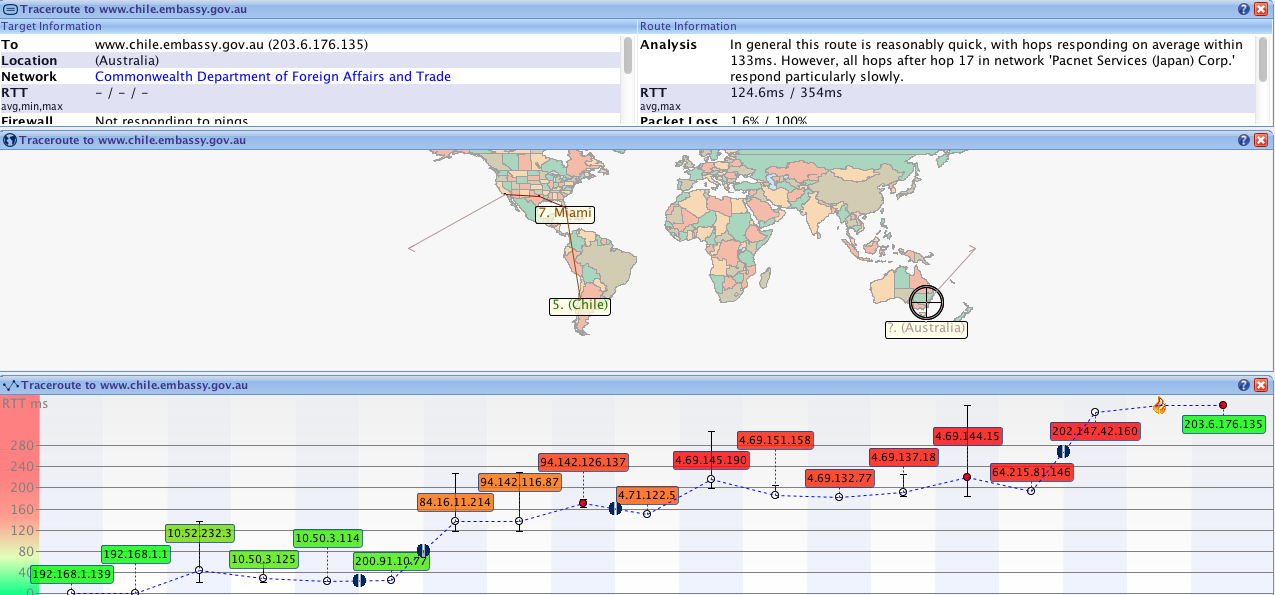
\includegraphics[width=1\textwidth]{au2}
  \caption{Embajada Australia en Chile}
  \label{fig:Trace Route de http://www.chile.embassy.gov.au/}
\end{figure}

Con respecto al camino que toman los paquetes, nuevamente, se observa que una vez fuera de territorio nacional, las latencias en los tiempos de respuesta aumenta (color naranja o rojo), a pesar de que se escoge la ruta menos congestionada.

\pagebreak

\subsection{http://google.cl/}

\pagebreak

\section{Algoritmo Vector-Distancia v1}
 
Para la realización de este ejercicio, se creo un tabla de $nxn$ en la cual se consideran los costos de cada router hacia sus vecinos en cada iteración. Para los vecinos en los cuales no se consiga llegar, se utilizó la simbología $\infty$, lo que significa que el costo para llegar a ese router, es tan alto que no se puede conseguir. 

Para el cálculo de cada costo, se utilizo la formula entregada en las diapositivas de clases, las cuales son :

$$D_u(z)=min\{c(u,v)+d_v(z)\}$$

Lo cúal se repite para cada nodo con sus vecinos. A medida que se avanza en las iteraciones, el alcanze desde un router hacia otro va aumentando en 1 por cada una de estas. Este algoritmo finaliza cuando los resultados de cada costo, convergen en los mismo resultados, dando asi cierta seguridad de que los costos son los mínimos.

Iteracón inicial, se consideran los caminos directos a los routers vecino que se puede alcanzar, por lo tanto la tabla que incluye cada tabla individual de costos para cada router, incluyendo el computador y el servidor:

\begin{table}[h]
\centering
\begin{tabular}{lclclclclclclclclclclc}

& PC & A & B & C & D & E & F & G & H & I & Server \\\hline\\
PC&0&3&$\infty$&$\infty$&$\infty$&$\infty$&$\infty$&$\infty$&$\infty$&$\infty$&$\infty$ \\
A&3&0&1&$\infty$&$\infty$&$\infty$&$\infty$&$\infty$&$\infty$&10&$\infty$ \\
B&$\infty$&1&0&9&$\infty$&8&$\infty$&$\infty$&$\infty$&$\infty$&$\infty$ \\
C&$\infty$&$\infty$&9&0&2&$\infty$&$\infty$&$\infty$&$\infty$&$\infty$&$\infty$ \\
D&$\infty$&$\infty$&$\infty$&2&0&9&9&$\infty$&$\infty$&$\infty$&$\infty$ \\
E&$\infty$&$\infty$&8&$\infty$&9&0&2&$\infty$&$\infty$&$\infty$&$\infty$ \\
F&$\infty$&$\infty$&$\infty$&$\infty$&9&2&0&$\infty$&6&$\infty$&$\infty$ \\
G&$\infty$&4&$\infty$&$\infty$&$\infty$&$\infty$&$\infty$&0&7&$\infty$&$\infty$ \\
H&$\infty$&$\infty$&$\infty$&$\infty$&$\infty$&$\infty$&6&7&0&3&$\infty$ \\
I&$\infty$&10&$\infty$&$\infty$&2&1&$\infty$&$\infty$&3&0&1 \\
Server&$\infty$&$\infty$&$\infty$&$\infty$&$\infty$&$\infty$&$\infty$&$\infty$&$\infty$&1&0 \\

\end{tabular}
\caption{\label{tab:widgets}Costos de cada router, para iteración inicial.}
\end{table}

\pagebreak
 

Para la siguiente iteración, se utilizó la ecuacion antes mencionada, generando la tabla, usando hasta dos routers para llegar a los vecinos.

\begin{table}[h]
\centering
\begin{tabular}{lclclclclclclclclclclc}

& PC & A & B & C & D & E & F & G & H & I & Server \\\hline\\
PC&0&3&4&$\infty$&$\infty$&$\infty$&$\infty$&7&$\infty$&13&$\infty$ \\
A&3&0&1&10&12&11&$\infty$&4&11&10&11 \\
B&4&1&0&9&11&8&10&5&$\infty$&9&$\infty$ \\
C&$\infty$&10&9&0&2&11&$\infty$&$\infty$&$\infty$&4&$\infty$ \\
D&$\infty$&12&11&2&0&3&9&$\infty$&5&2&3 \\
E&$\infty$&11&8&11&3&0&2&$\infty$&4&1&2 \\
F&$\infty$&$\infty$&10&$\infty$&9&2&0&13&6&3&$\infty$ \\
G&7&4&5&$\infty$&$\infty$&$\infty$&13&0&7&10&$\infty$ \\
H&$\infty$&11&$\infty$&$\infty$&5&4&6&7&0&3&4 \\
I&13&10&9&4&2&1&3&10&3&0&1 \\
Server&$\infty$&11&$\infty$&$\infty$&3&2&$\infty$&$\infty$&4&1&0 \\

\end{tabular}
\caption{\label{tab:widgets}Costos de cada router, para iteración primera.}
\end{table}

Se repite el proceso anterior, reduciendo costos $\infty$ y algunos otros generandos una matriz de costos menor, observandose en la tabla:

\begin{table}[h]
\centering
\begin{tabular}{lclclclclclclclclclclc}

& PC & A & B & C & D & E & F & G & H & I & Server \\\hline\\
PC&0&3&4&13&12&11&14&7&14&13&14 \\
A&3&0&1&10&12&9&11&4&11&10&11 \\
B&4&1&0&9&11&8&10&5&12&9&10 \\
C&13&10&9&0&2&5&7&14&7&4&5 \\
D&15&12&11&2&0&3&5&12&5&2&3 \\
E&14&9&8&5&3&0&2&13&4&1&2 \\
F&16&11&10&7&5&2&0&13&6&3&4 \\
G&7&4&5&14&12&11&13&0&7&10&11 \\
H&14&11&12&7&5&4&6&7&0&3&4 \\
I&13&10&9&4&2&1&3&10&3&0&1 \\
Server&14&11&10&5&3&2&4&11&4&1&0 \\

\end{tabular}
\caption{\label{tab:widgets}Costos de cada router, para iteración 2.}
\end{table}
 
En la iteración 3, notamos que los resultados se repiten a pesar de que la cantidad de routeres por los que podemos pasar aumenta, luego notamos que existe convergencia en los resultados. Los resutlados se ven en la siguiente tabla:

\begin{table}[h]
\centering
\begin{tabular}{lclclclclclclclclclclc}

& PC & A & B & C & D & E & F & G & H & I & Server \\\hline\\
PC&0&3&4&13&12&11&14&7&14&13&14 \\
A&3&0&1&10&12&9&11&4&11&10&11 \\
B&4&1&0&9&11&8&10&5&12&9&10 \\
C&13&10&9&0&2&5&7&14&7&4&5 \\
D&15&12&11&2&0&3&5&12&5&2&3 \\
E&14&9&8&5&3&0&2&13&4&1&2 \\
F&16&11&10&7&5&2&0&13&6&3&4 \\
G&7&4&5&14&12&11&13&0&7&10&11 \\
H&14&11&12&7&5&4&6&7&0&3&4 \\
I&13&10&9&4&2&1&3&10&3&0&1 \\
Server&14&11&10&5&3&2&4&11&4&1&0 \\

\end{tabular}
\caption{\label{tab:widgets}Costos de cada router, para iteración 3.}
\end{table}
\pagebreak

\section{Algoritmo Vector-Distancia v2}
 
En este caso, se corta la conexion entre los Routers H e I, lo que produce una matriz de costos diferente a la de la parte anterior, la cual se muestra en la siguiente tabla:


\begin{table}[h]
\centering
\begin{tabular}{lclclclclclclclclclclc}

& PC & A & B & C & D & E & F & G & H & I & Server \\\hline\\
PC&0&3&$\infty$&$\infty$&$\infty$&$\infty$&$\infty$&$\infty$&$\infty$&$\infty$&$\infty$ \\
A&3&0&1&$\infty$&$\infty$&$\infty$&$\infty$&$\infty$&$\infty$&10&$\infty$ \\
B&$\infty$&1&0&9&$\infty$&8&$\infty$&$\infty$&$\infty$&$\infty$&$\infty$ \\
C&$\infty$&$\infty$&9&0&2&$\infty$&$\infty$&$\infty$&$\infty$&$\infty$&$\infty$ \\
D&$\infty$&$\infty$&$\infty$&2&0&9&9&$\infty$&$\infty$&$\infty$&$\infty$ \\
E&$\infty$&$\infty$&8&$\infty$&9&0&2&$\infty$&$\infty$&$\infty$&$\infty$ \\
F&$\infty$&$\infty$&$\infty$&$\infty$&9&2&0&$\infty$&6&$\infty$&$\infty$ \\
G&$\infty$&4&$\infty$&$\infty$&$\infty$&$\infty$&$\infty$&0&7&$\infty$&$\infty$ \\
H&$\infty$&$\infty$&$\infty$&$\infty$&$\infty$&$\infty$&6&7&0&$\infty$&$\infty$ \\
I&$\infty$&10&$\infty$&$\infty$&2&1&$\infty$&$\infty$&$\infty$&0&1 \\
Server&$\infty$&$\infty$&$\infty$&$\infty$&$\infty$&$\infty$&$\infty$&$\infty$&$\infty$&1&0 \\

\end{tabular}
\caption{\label{tab:widgets}Costos de cada router, para iteración inicial para conexión cortada.}
\end{table}
 
Luego, si repetimos el proceso anterior, en la siguiente iteración generamos la siguiente tabla de costos, sin utilizar la conexion $h-i$, notar que aparecen mas costos $\infty$, lo que va mostrando ciertas consecuencias de cortar las conexiones entre dos routers en cierto momento:
\pagebreak

\begin{table}[h]
\centering
\begin{tabular}{lclclclclclclclclclclc}

& PC & A & B & C & D & E & F & G & H & I & Server \\\hline\\
PC&0&3&4&$\infty$&$\infty$&$\infty$&$\infty$&7&$\infty$&13&$\infty$ \\
A&3&0&1&10&12&11&$\infty$&4&11&10&11 \\
B&4&1&0&9&11&8&10&5&$\infty$&9&$\infty$ \\
C&$\infty$&10&9&0&2&11&$\infty$&$\infty$&$\infty$&4&$\infty$ \\
D&$\infty$&12&11&2&0&3&9&$\infty$&$\infty$&2&3 \\
E&$\infty$&11&8&11&3&0&2&$\infty$&8&1&2 \\
F&$\infty$&$\infty$&10&$\infty$&9&2&0&13&6&3&$\infty$ \\
G&7&4&5&$\infty$&$\infty$&$\infty$&13&0&7&$\infty$&$\infty$ \\
H&$\infty$&11&$\infty$&$\infty$&$\infty$&8&6&7&0&$\infty$&$\infty$ \\
I&13&10&9&4&2&1&$\infty$&$\infty$&$\infty$&0&1 \\
Server&$\infty$&11&$\infty$&$\infty$&3&2&$\infty$&$\infty$&$\infty$&1&0 \\

\end{tabular}
\caption{\label{tab:widgets}Costos de cada router, para iteración primera.}
\end{table}

Para la siguiente iteración aun aparecen costos $\infty$, por lo que debemos seguir iterando: 

\begin{table}[h]
\centering
\begin{tabular}{lclclclclclclclclclclc}

& PC & A & B & C & D & E & F & G & H & I & Server \\\hline\\
PC&0&3&4&13&12&11&14&7&14&13&14 \\
A&3&0&1&10&12&9&11&4&11&10&11 \\
B&4&1&0&9&11&8&10&5&12&9&10 \\
C&13&10&9&0&2&5&7&14&7&4&5 \\
D&15&12&11&2&0&3&5&12&15&2&3 \\
E&14&9&8&5&3&0&2&13&8&1&2 \\
F&16&11&10&7&5&2&0&13&6&3&4 \\
G&7&4&5&14&12&11&13&0&7&14&11 \\
H&14&11&12&7&15&8&6&7&0&9&$\infty$ \\
I&13&10&9&4&2&1&3&14&9&0&1 \\
Server&14&11&10&5&3&2&4&11&$\infty$&1&0 \\

\end{tabular}
\caption{\label{tab:widgets}Costos de cada router, para iteración 2.}
\end{table}

La siguiente iteración logra eliminar los costos $\infty$, obteniendose la siguiente tabla de costos:

\pagebreak

\begin{table}[h]
\centering
\begin{tabular}{lclclclclclclclclclclc}

& PC & A & B & C & D & E & F & G & H & I & Server \\\hline\\
PC&0&3&4&13&12&11&14&7&14&13&14 \\
A&3&0&1&10&12&9&11&4&11&10&11 \\
B&4&1&0&9&11&8&10&5&12&9&10 \\
C&13&10&9&0&2&5&7&14&7&4&5 \\
D&15&12&11&2&0&3&5&12&11&2&3 \\
E&14&9&8&5&3&0&2&13&4&1&2 \\
F&16&11&10&7&5&2&0&13&6&3&4 \\
G&7&4&5&14&12&11&13&0&7&10&11 \\
H&14&11&12&7&11&4&6&7&0&3&10 \\
I&13&10&9&4&2&1&3&10&3&0&1 \\
Server&14&11&10&5&3&2&4&11&10&1&0 \\

\end{tabular}
\caption{\label{tab:widgets}Costos de cada router, para iteración 3.}
\end{table}

Al iterar nuevamente, obtenemos los mismos valores de la tabla anterior, por lo tanto logramos convergencia en los valores de costos, lo que nos permite aseguirar que son los valores definitivos:

\begin{table}[h]
\centering
\begin{tabular}{lclclclclclclclclclclc}

& PC & A & B & C & D & E & F & G & H & I & Server \\\hline\\
PC&0&3&4&13&12&11&14&7&14&13&14 \\
A&3&0&1&10&12&9&11&4&11&10&11 \\
B&4&1&0&9&11&8&10&5&12&9&10 \\
C&13&10&9&0&2&5&7&14&7&4&5 \\
D&15&12&11&2&0&3&5&12&11&2&3 \\
E&14&9&8&5&3&0&2&13&4&1&2 \\
F&16&11&10&7&5&2&0&13&6&3&4 \\
G&7&4&5&14&12&11&13&0&7&10&11 \\
H&14&11&12&7&11&4&6&7&0&3&10 \\
I&13&10&9&4&2&1&3&10&3&0&1 \\
Server&14&11&10&5&3&2&4&11&10&1&0 \\

\end{tabular}
\caption{\label{tab:widgets}Costos de cada router, para iteración 4.}
\end{table}

Finalmente notamos que los costos aumentaron en algunos de los caminos entre routers, pero no afectando el costo minimo entre el PC y el Servidor, manteniendose en 14.


\end{document}